% This is "sig-alternate.tex" V2.1 April 2013
% This file should be compiled with V2.5 of "sig-alternate.cls" May 2012
%
% This example file demonstrates the use of the 'sig-alternate.cls'
% V2.5 LaTeX2e document class file. It is for those submitting
% articles to ACM Conference Proceedings WHO DO NOT WISH TO
% STRICTLY ADHERE TO THE SIGS (PUBS-BOARD-ENDORSED) STYLE.
% The 'sig-alternate.cls' file will produce a similar-looking,
% albeit, 'tighter' paper resulting in, invariably, fewer pages.
%
% ----------------------------------------------------------------------------------------------------------------
% This .tex file (and associated .cls V2.5) produces:
%       1) The Permission Statement
%       2) The Conference (location) Info information
%       3) The Copyright Line with ACM data
%       4) NO page numbers
%
% as against the acm_proc_article-sp.cls file which
% DOES NOT produce 1) thru' 3) above.
%
% Using 'sig-alternate.cls' you have control, however, from within
% the source .tex file, over both the CopyrightYear
% (defaulted to 200X) and the ACM Copyright Data
% (defaulted to X-XXXXX-XX-X/XX/XX).
% e.g.
% \CopyrightYear{2007} will cause 2007 to appear in the copyright line.
% \crdata{0-12345-67-8/90/12} will cause 0-12345-67-8/90/12 to appear in the copyright line.
%
% ---------------------------------------------------------------------------------------------------------------
% This .tex source is an example which *does* use
% the .bib file (from which the .bbl file % is produced).
% REMEMBER HOWEVER: After having produced the .bbl file,
% and prior to final submission, you *NEED* to 'insert'
% your .bbl file into your source .tex file so as to provide
% ONE 'self-contained' source file.
%
% ================= IF YOU HAVE QUESTIONS =======================
% Questions regarding the SIGS styles, SIGS policies and
% procedures, Conferences etc. should be sent to
% Adrienne Griscti (griscti@acm.org)
%
% Technical questions _only_ to
% Gerald Murray (murray@hq.acm.org)
% ===============================================================
%
% For tracking purposes - this is V2.0 - May 2012

\documentclass{sig-alternate-05-2015}

\begin{document}

% Copyright
\setcopyright{acmcopyright}
%\setcopyright{acmlicensed}
%\setcopyright{rightsretained}
%\setcopyright{usgov}
%\setcopyright{usgovmixed}
%\setcopyright{cagov}
%\setcopyright{cagovmixed}


% DOI
\doi{10.475/123_4}

% ISBN
\isbn{123-4567-24-567/08/06}

%Conference
\conferenceinfo{PLDI '13}{June 16--19, 2013, Seattle, WA, USA}

\acmPrice{\$15.00}

%
% --- Author Metadata here ---
\conferenceinfo{WOODSTOCK}{'97 El Paso, Texas USA}
%\CopyrightYear{2007} % Allows default copyright year (20XX) to be over-ridden - IF NEED BE.
%\crdata{0-12345-67-8/90/01}  % Allows default copyright data (0-89791-88-6/97/05) to be over-ridden - IF NEED BE.
% --- End of Author Metadata ---

\title{Feature Usage In Java\titlenote{For use with
SIG-ALTERNATE.CLS. Supported by ACM.}}
%\subtitle{[Extended Abstract]
%\titlenote{A full version of this paper is available as
%\textit{Author's Guide to Preparing ACM SIG Proceedings Using
%\LaTeX$2_\epsilon$\ and BibTeX} at
%\texttt{www.acm.org/eaddress.htm}}}
%
% You need the command \numberofauthors to handle the 'placement
% and alignment' of the authors beneath the title.
%
% For aesthetic reasons, we recommend 'three authors at a time'
% i.e. three 'name/affiliation blocks' be placed beneath the title.
%
% NOTE: You are NOT restricted in how many 'rows' of
% "name/affiliations" may appear. We just ask that you restrict
% the number of 'columns' to three.
%
% Because of the available 'opening page real-estate'
% we ask you to refrain from putting more than six authors
% (two rows with three columns) beneath the article title.
% More than six makes the first-page appear very cluttered indeed.
%
% Use the \alignauthor commands to handle the names
% and affiliations for an 'aesthetic maximum' of six authors.
% Add names, affiliations, addresses for
% the seventh etc. author(s) as the argument for the
% \additionalauthors command.
% These 'additional authors' will be output/set for you
% without further effort on your part as the last section in
% the body of your article BEFORE References or any Appendices.

\numberofauthors{8} %  in this sample file, there are a *total*
% of EIGHT authors. SIX appear on the 'first-page' (for formatting
% reasons) and the remaining two appear in the \additionalauthors section.
%
\author{
% You can go ahead and credit any number of authors here,
% e.g. one 'row of three' or two rows (consisting of one row of three
% and a second row of one, two or three).
%
% The command \alignauthor (no curly braces needed) should
% precede each author name, affiliation/snail-mail address and
% e-mail address. Additionally, tag each line of
% affiliation/address with \affaddr, and tag the
% e-mail address with \email.
%
% 1st. author
\alignauthor
Michael Feist\\
       \affaddr{University of Alberta}\\
       \email{mdfeist@ualberta.ca}
% 2nd. author
\alignauthor
Ian Watts\\
       \affaddr{University of Alberta}\\
       \email{watts@ualberta.ca}
% 3rd. author
% Leaving this here in case we need to include Abram Hindle
\alignauthor Lars Th{\o}rv{\"a}ld\\
       \affaddr{The Th{\o}rv{\"a}ld Group}\\
       \affaddr{1 Th{\o}rv{\"a}ld Circle}\\
       \affaddr{Hekla, Iceland}\\
       \email{larst@affiliation.org}
\and  % use '\and' if you need 'another row' of author names
}


\maketitle
\begin{abstract}
A Java project contains many different types which are defined by the language, the developers and included libraries. This paper examines how many of those types are being used by developers in Java projects. A tool for computing the difference between Abstract Syntax Trees (AST) is used to compare revisions in GitHub repositories to find what libraries and types are contributed and changed by different authors. From these differences, the number of types used by an individual developer is calculated. A developer's exposure to different parts of a project is measured by how many out of the total number of types they have used. A comparison between developers is used to see if programmers specialize type usage in their contributions. We find that most projects use a large number of types and most developers only touched a small portion of the total types. We also propose the use of this metric to encourage developers to increase their exposure to more parts of a project.

\end{abstract}


%
% The code below should be generated by the tool at
% http://dl.acm.org/ccs.cfm
% Please copy and paste the code instead of the example below. 
%

%Not sure what key words to use here
\begin{CCSXML}
<ccs2012>
<concept>
<concept_id>10011007.10010940</concept_id>
<concept_desc>Software and its engineering~Software organization and properties</concept_desc>
<concept_significance>300</concept_significance>
</concept>
</ccs2012>
\end{CCSXML}

\ccsdesc[300]{Software and its engineering~Software organization and properties}


%
% End generated code
%

%
%  Use this command to print the description
%
\printccsdesc

% We no longer use \terms command
%\terms{Theory}

\keywords{Software Engineering; Mining Software Repositories; Programming Languages; Abstract Syntax Trees}

\section{Introduction}
Language features
A programming language contains many constructs and features to allow the programmer to 
complete a task in an effective manner. However, most tasks can be complteded
while only using a small subset of these features (reference).

Behaviour of developers
Beginner developers use less features(ref)?
As a developers experience with a language increases... Use more features

Abstract Syntax Trees
An Abstract Syntax Tree (AST) is a tree structrure which represents the 
language constructs contained in a file. Each node in the tree... 
Each child in the tree...
Comparison of two trees

In this paper we will attempt to answer the following research questions:
RQ1:



\section{Related Works}
General Description of prior work

Paper 1 has ...
Use of java language features over time.
 There are millions of places features could potentially be used but weren't. 
Developers convert existing code to use new features
They found thousands of instances of potential resource handling bugs.
Are the use of languages anticipated? 
Are they being used before the release date?
Some features widely used, others not so much
Due to lack of opportunity? Check for situations before and after release of feature
Need better tools or training to promote use of features
Most popular features: annotation use, enhanced-for loops, and variables with generic types
Team vs individual adoption rate of new features
PER COMMITER use of features
First person to commit a feature is marked as having used that feature

Paper 2 has ...



\section{Methodology}
Describe AST diff tools, histogram of constructs

\subsection{Metric}

\subsection{Data Set}
Our data set consists of 216 Github repositories. To ensure that we only look at Java repositories of reasonable size we first queried BOA \cite{Dyer-Nguyen-Rajan-Nguyen-13} for eligible repositories. We ran our BOA query over the 2015 Github September dataset. The criteria for a repository to be accept was that it include at least 10 Java files, 3 different committers, 30 commits, and at least one commit from after 2014. This allowed us to narrow our search down to sizable Java projects that were recently active. Out of the possible repositories returned from BOA we randomly chose the 216 repositories and pulled them from Github.

\subsection{Approach}
To determine what types in a project an author declared we looked at all revisions in each of the 216 Github repositories. Using the Gumtree algorithm with Spoon \cite{falleri:hal-01054552} we were able to generate ASTs for each of the differences between the revisions. Next we only looked at additions and modifications as deletions do not necessarily show that an author is using that type. We then counted the number of times a type is declared in the ASTs. By adding up the types used by each author in a given project we were able to determine the total number of types used in each project. This then allowed us to calculate the percent of types an author modified or added compared to the total number of types in a project.

\section{Analysis and Findings}
We found that more than half of the projects used less than 250 different types. But there were a few projects that used thousands of different types.

\begin{figure}[ht]
\centering
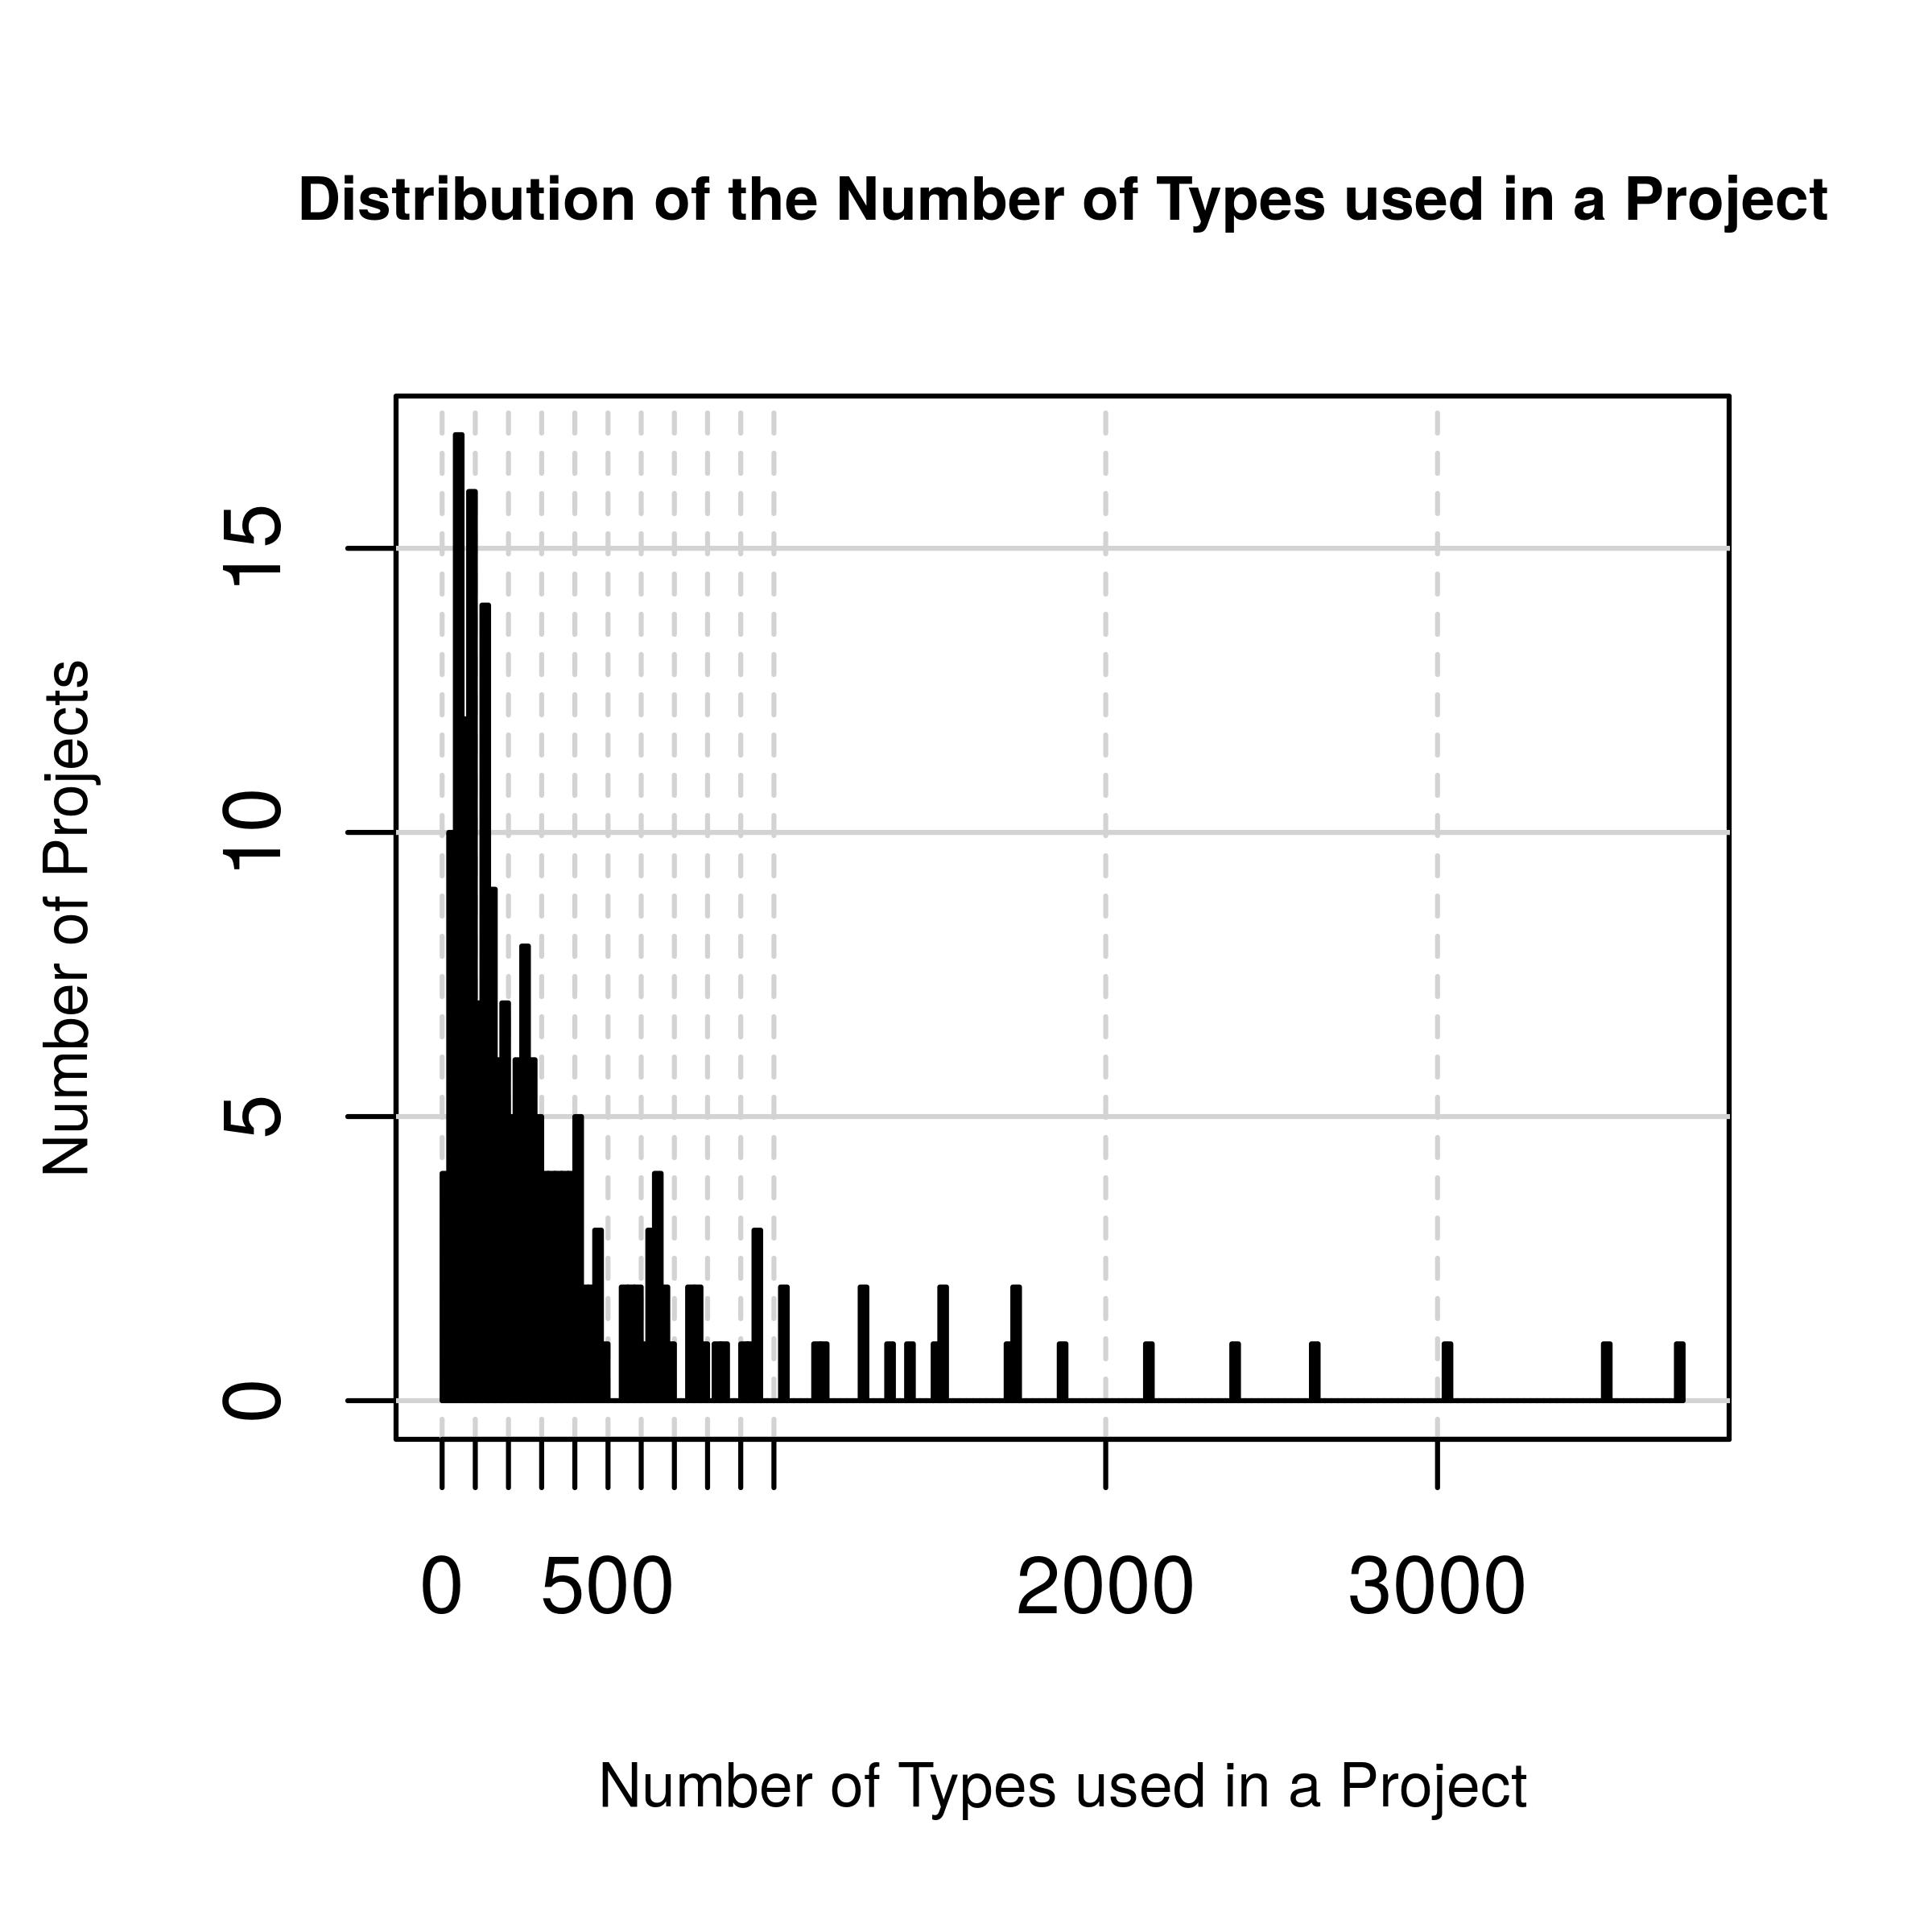
\includegraphics[height=3in, width=3in]{../lib_stats_number_of_libraries_dist}
\caption{A sample black and white graphic.}
\end{figure}

\subsection{RQ1: Do developers stick to the same types in a project?}

\begin{figure}[ht]
\centering
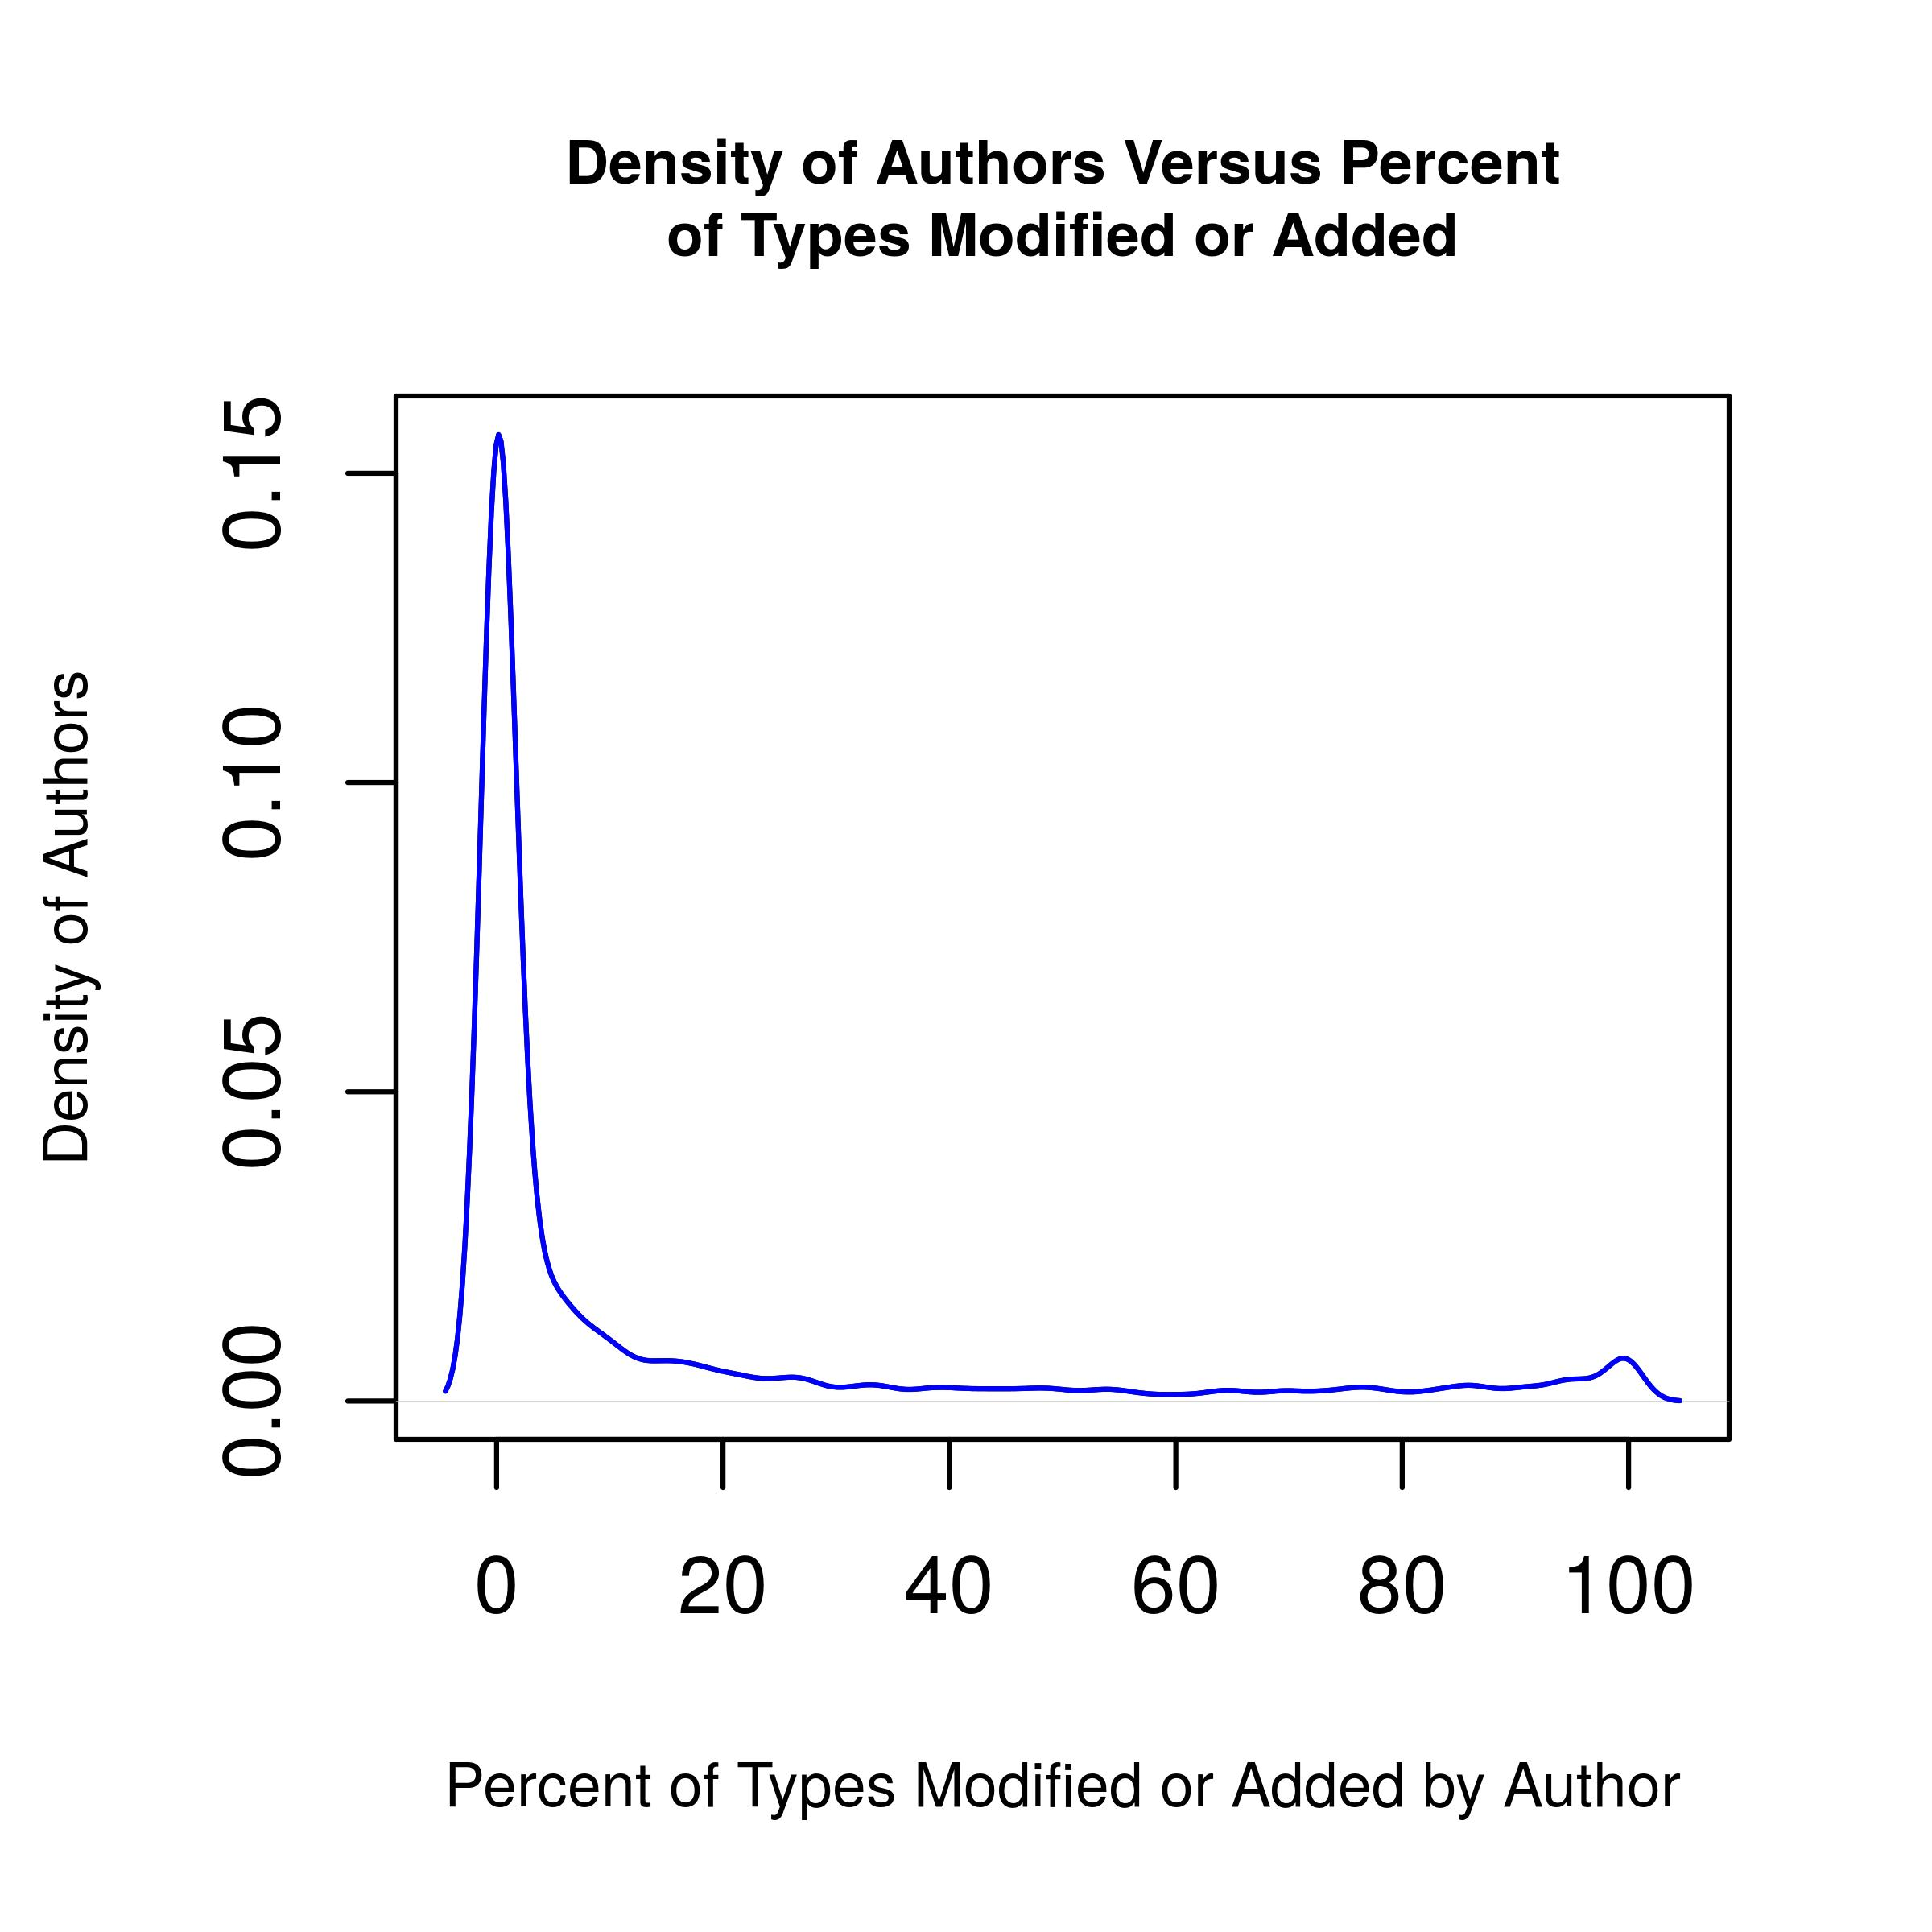
\includegraphics[height=3in, width=3in]{../lib_stats_dist}
\caption{A sample black and white graphic.}
\end{figure}

\begin{figure}[ht]
\centering
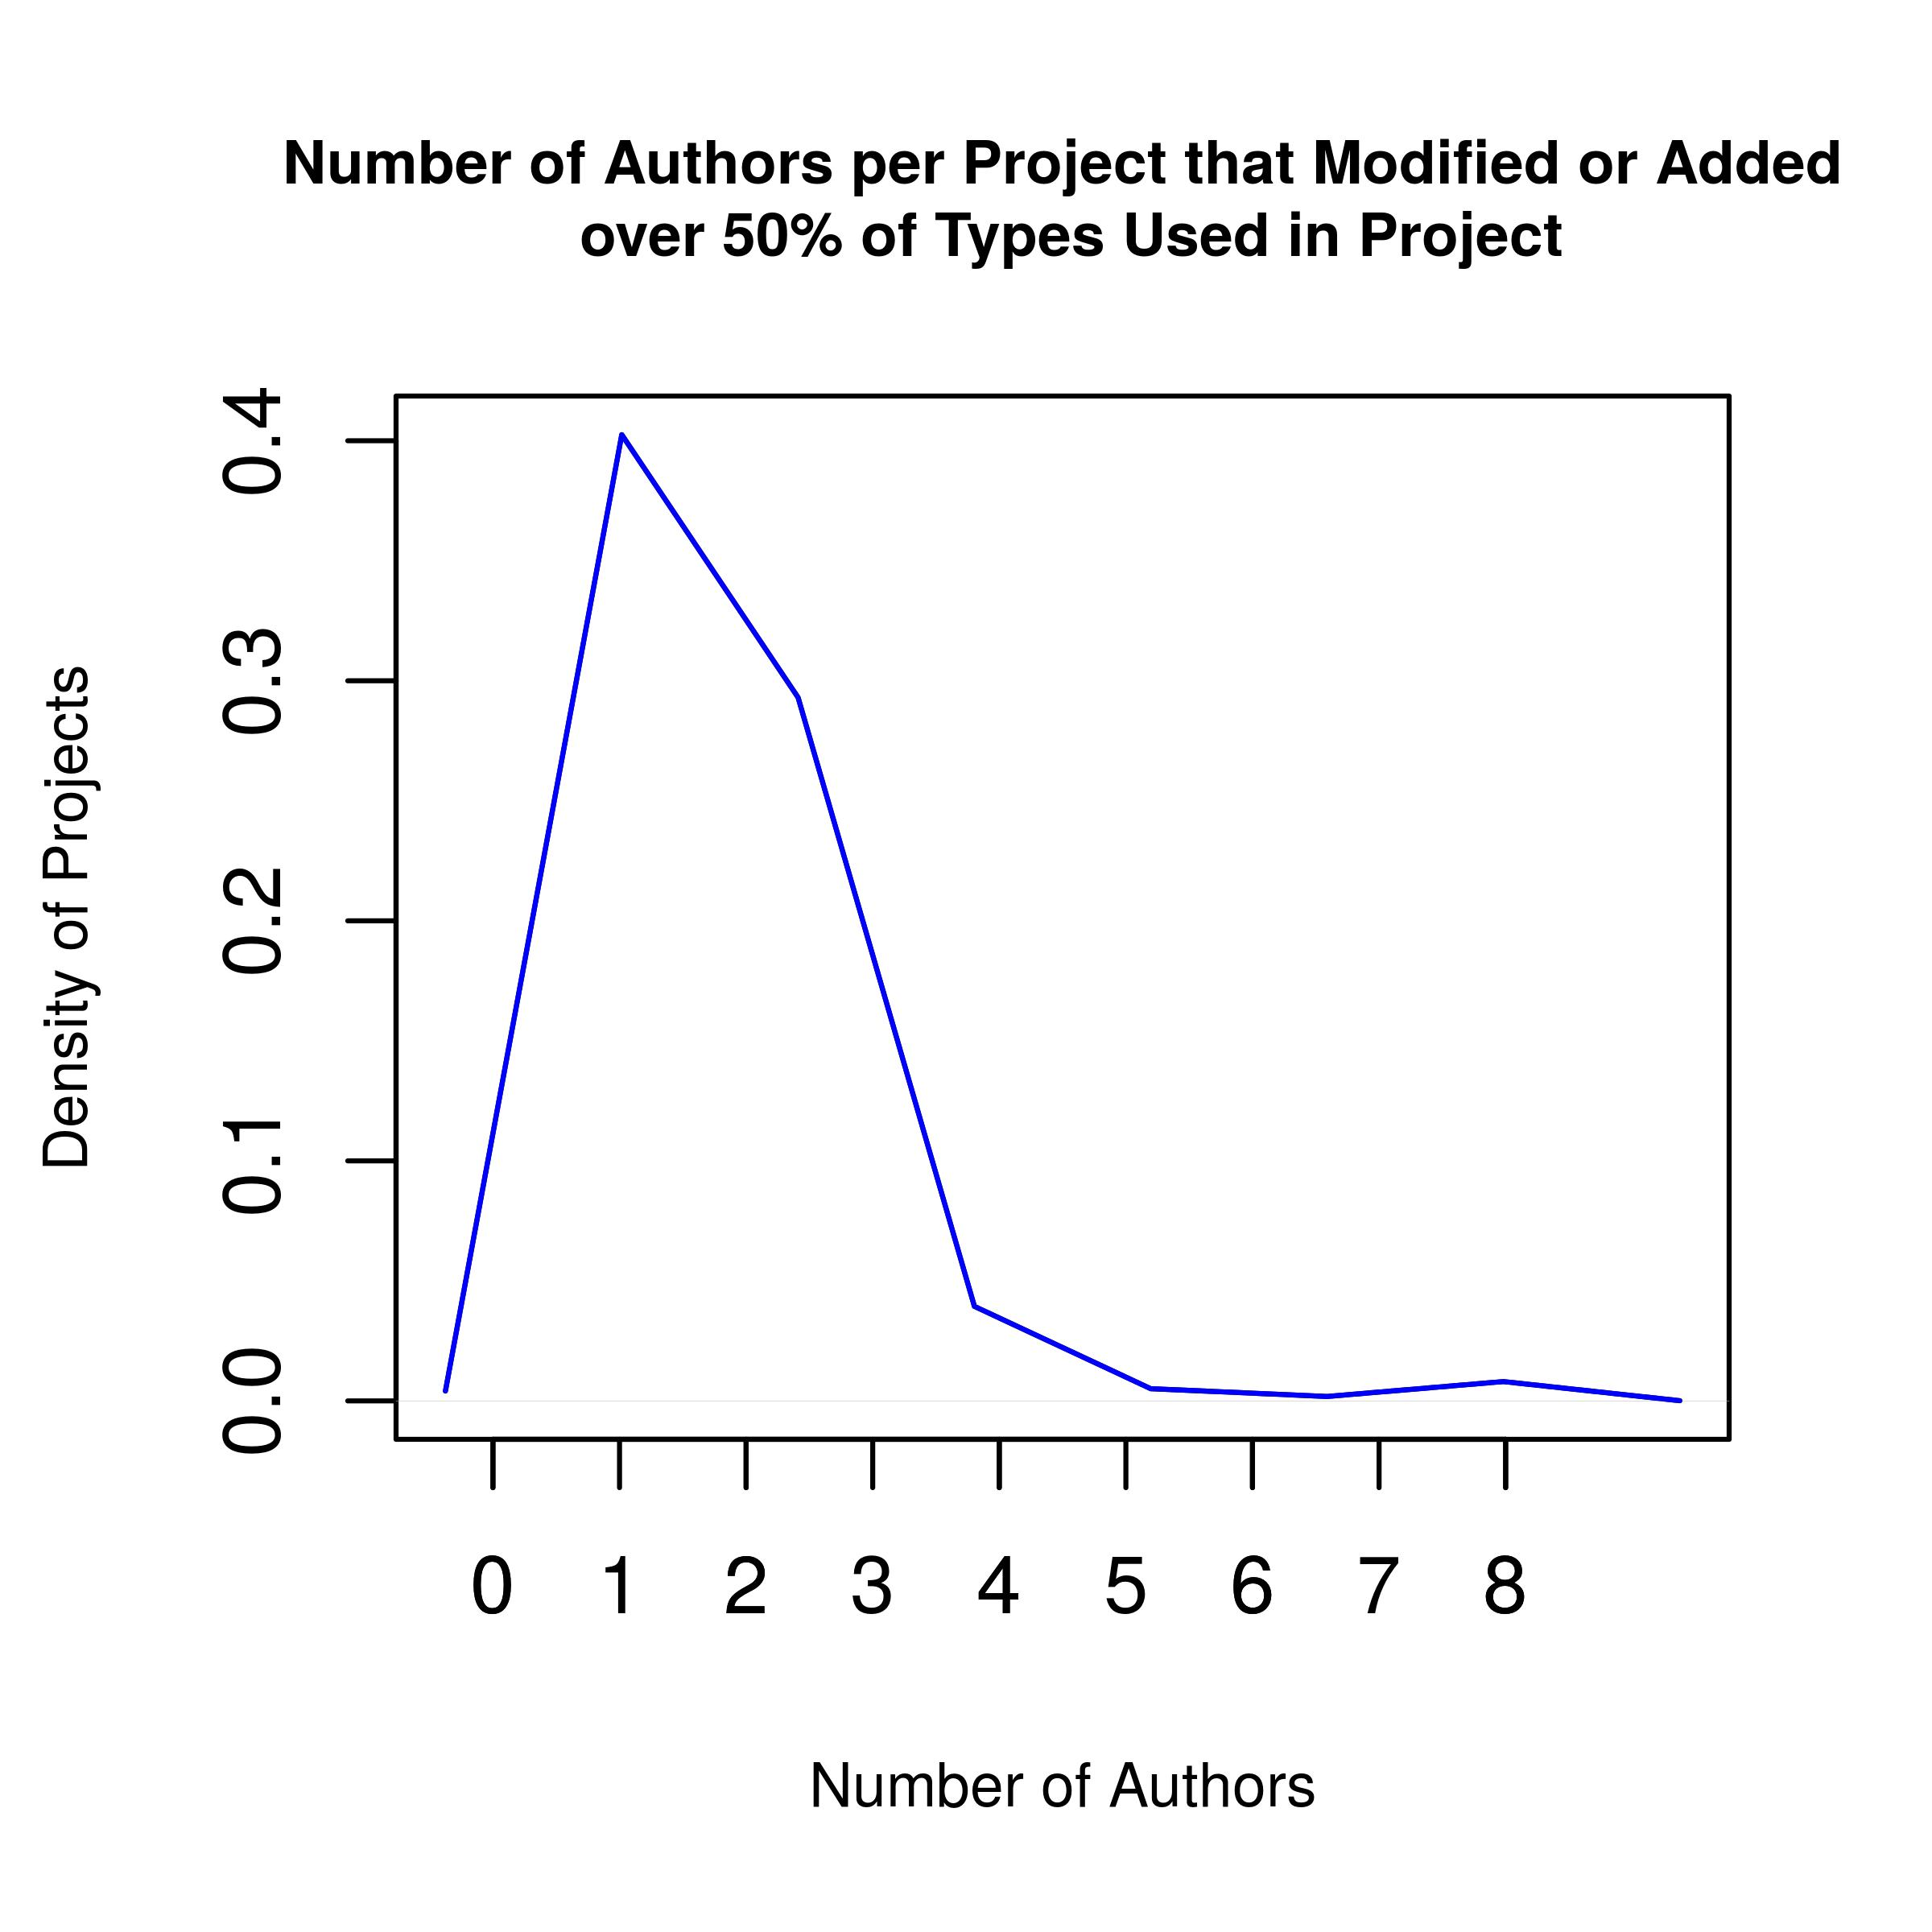
\includegraphics[height=3in, width=3in]{../lib_stats_Threshold50_dist}
\caption{A sample black and white graphic.}
\end{figure}

\begin{figure}[ht]
\centering
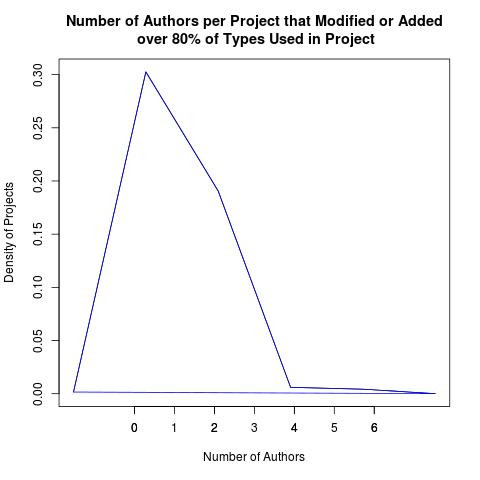
\includegraphics[height=3in, width=3in]{../lib_stats_Threshold80_dist}
\caption{A sample black and white graphic.}
\end{figure}

\subsection{RQ2: How many developers in each project had large coverages?}

\begin{figure}[ht]
\centering
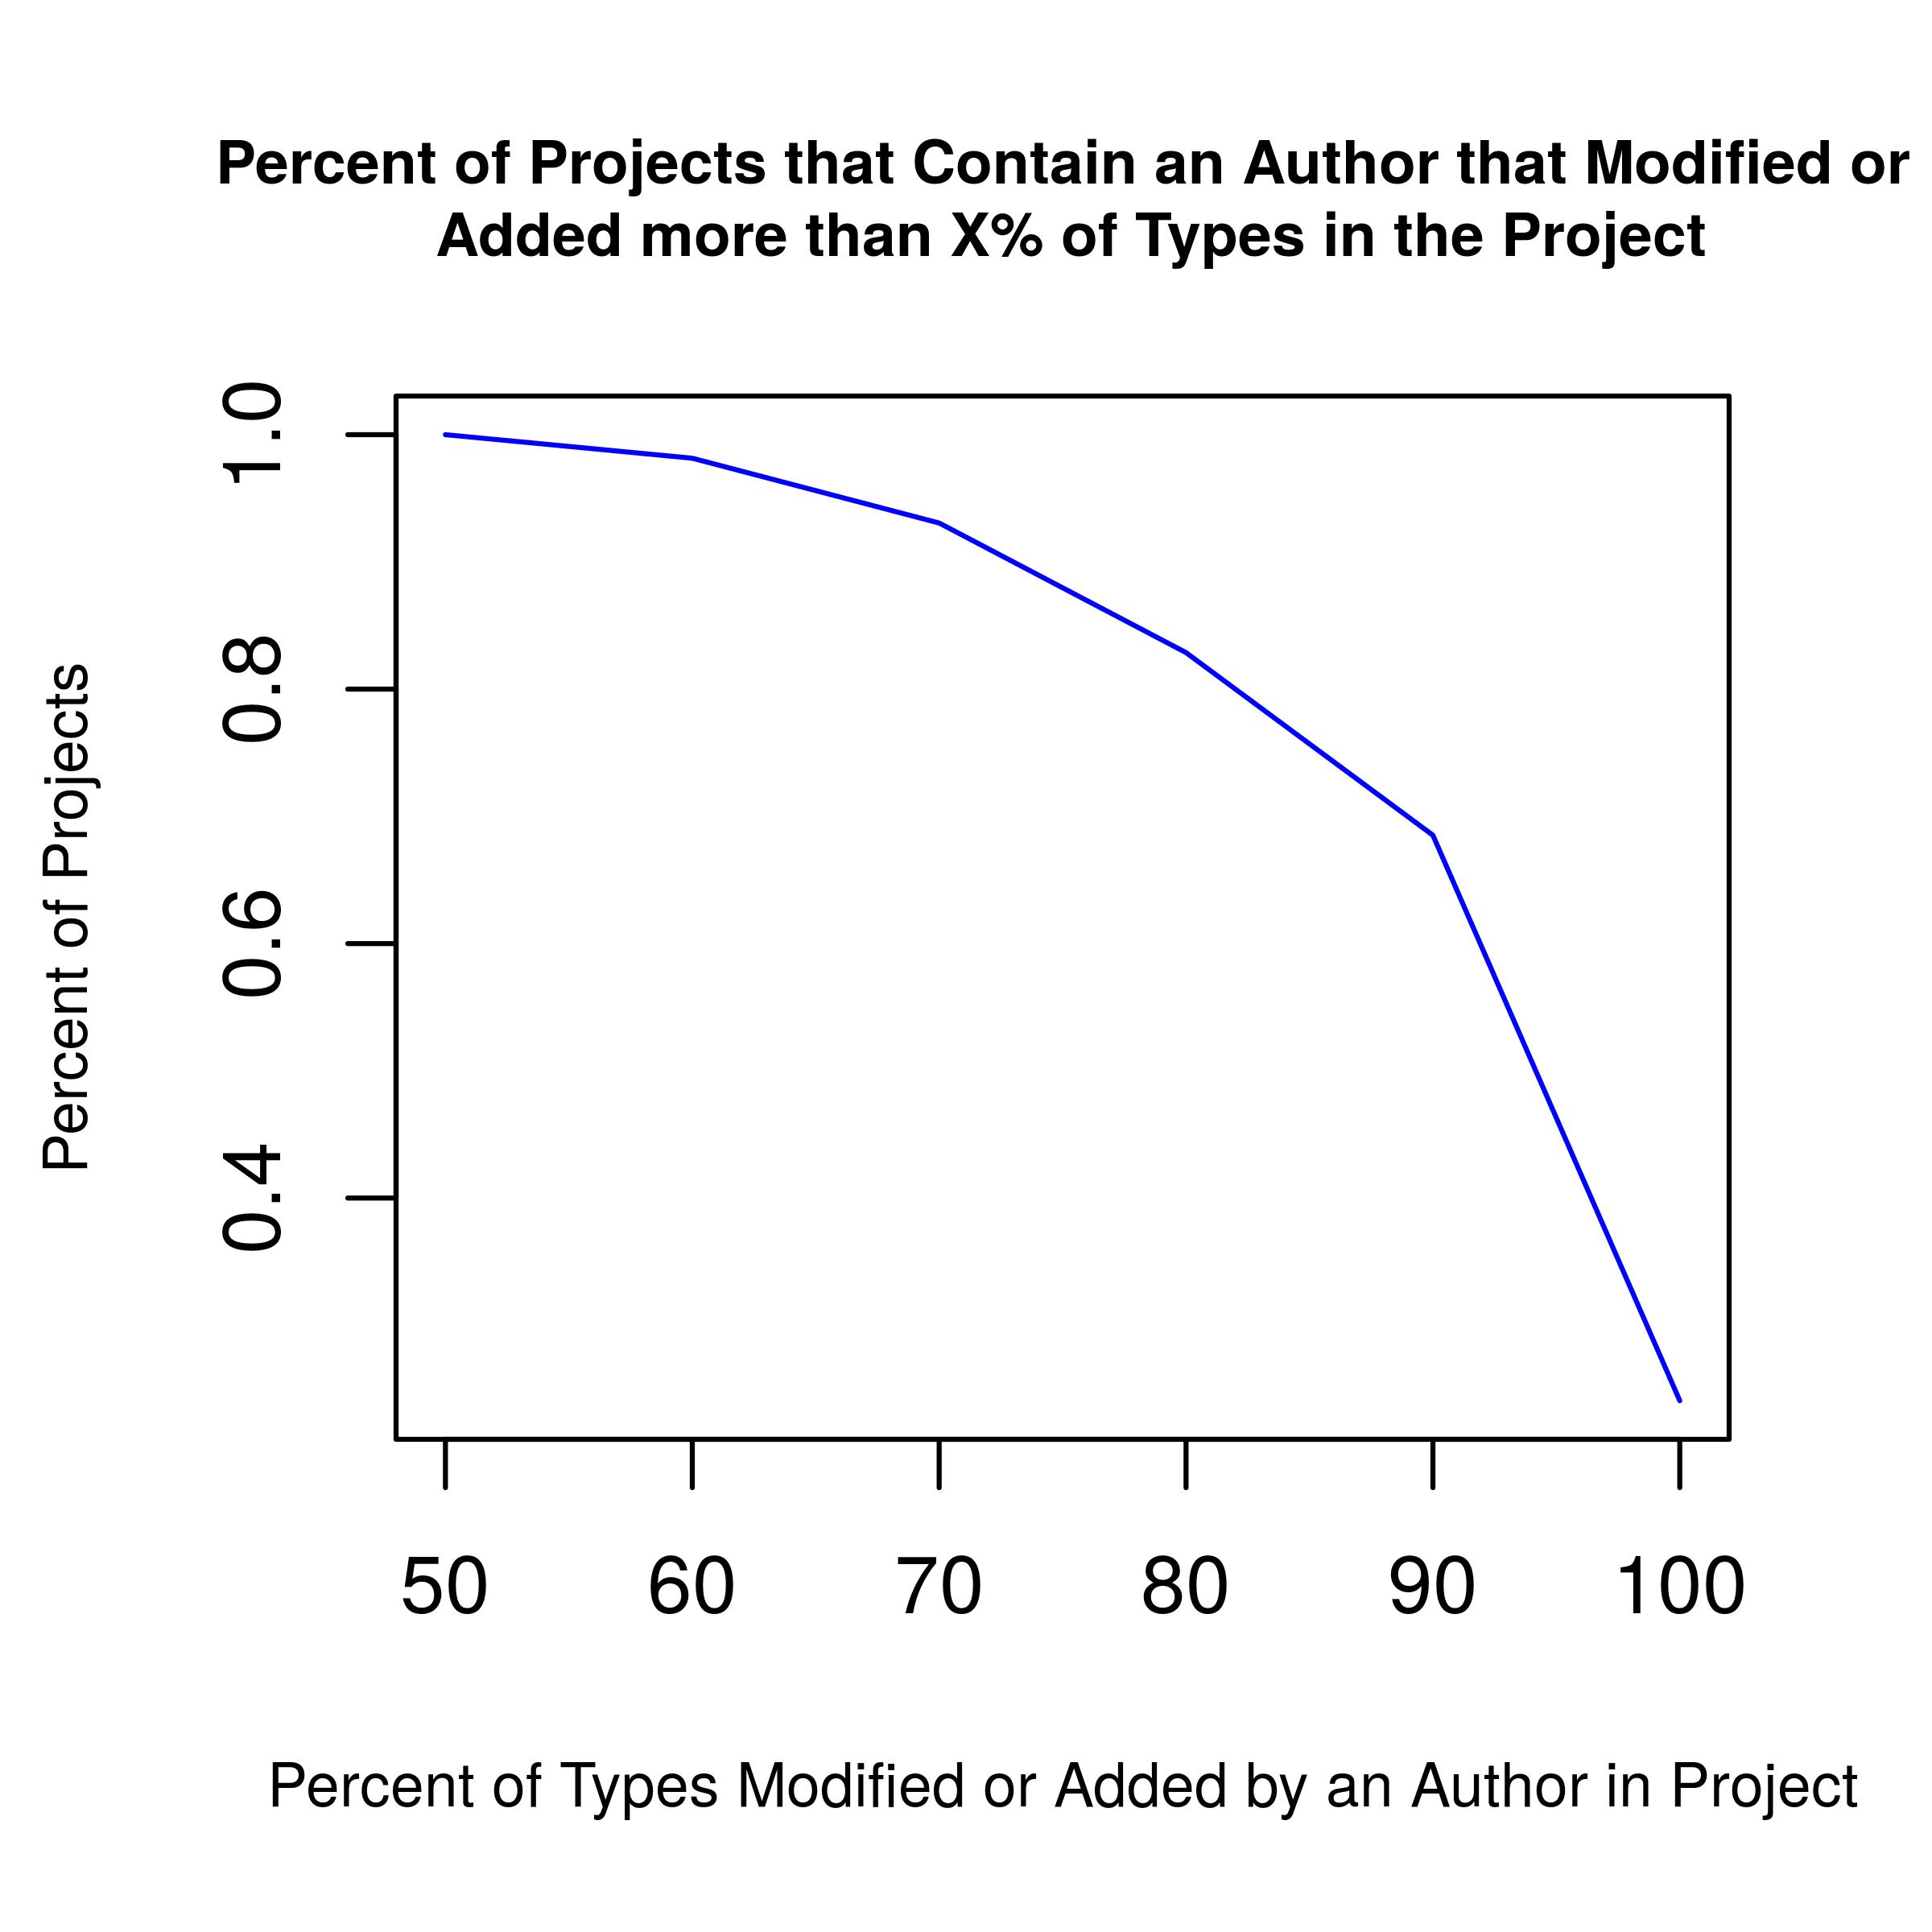
\includegraphics[height=3in, width=3in]{../lib_stats_count_authors_percent_per_project}
\caption{A sample black and white graphic.}
\end{figure}

\section{Conclusions and Future Work}
%\end{document}  % This is where a 'short' article might terminate

%ACKNOWLEDGMENTS are optional
\section{Acknowledgments}

%
% The following two commands are all you need in the
% initial runs of your .tex file to
% produce the bibliography for the citations in your paper.
\bibliographystyle{abbrv}
\bibliography{sigproc}  % sigproc.bib is the name of the Bibliography in this case
% You must have a proper ".bib" file
%  and remember to run:
% latex bibtex latex latex
% to resolve all references
%
% ACM needs 'a single self-contained file'!
%
%APPENDICES are optional
%\balancecolumns
\appendix
%Appendix A
\section{Headings in Appendices}

%\balancecolumns % GM June 2007
% That's all folks!
\end{document}
